\section{Path Tracing}
\label{sec:chapter_stato_arte_path_tracing}

In computer grafica, path tracing è una tecnica di rendering che fornisce una soluzione molto più realistica al problema del calcolo della luce rispetto al ray casting.
Il rendering che si ottiene mediante questo algoritmo è una vera simulazione di come la luce percorre la scena e non solamente una approssimazione artistica. Permette di simulare effetti quali ad esempio luci indirette come la luce che rimbalza da una superficie (Fig. \ref{fig:stato_arte_luci_dir_ind}), ombre leggere ed effetti caustici (Fig. \ref{fig:stato_arte_ombre_caust}) 
\\
\begin{figure}[htb]
 \centering
 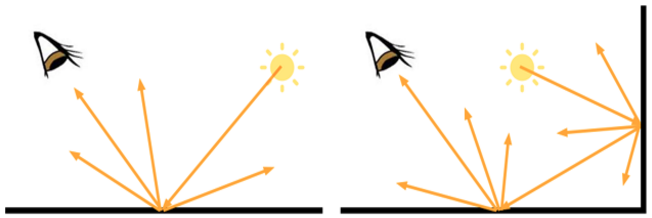
\includegraphics[width=0.8\linewidth]{images/chapter_stato_arte/stato_arte_luci_dir_ind.png}\hfill
 \caption[Illuminazione diretta e indiretta]{Confronto tra illuminazione diretta (a sinistra) e indiretta (a destra)}
 \label{fig:stato_arte_luci_dir_ind}
\end{figure}
\\
\begin{figure}[htb]
 \centering
 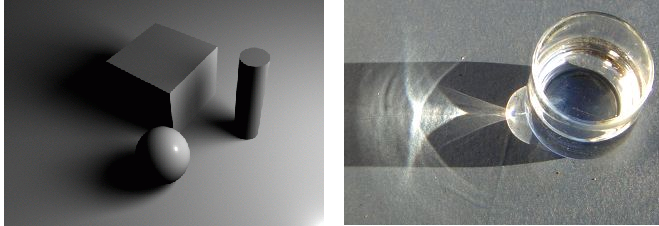
\includegraphics[width=0.8\linewidth]{images/chapter_stato_arte/stato_arte_ombre_caust.png}\hfill
 \caption[Ombreggiature ed effetti caustici]{Una scena con delle ombre leggere (a sinistra), ed effetti caustici nella realtà (a destra)}
 \label{fig:stato_arte_ombre_caust}
\end{figure}

L’ approccio utilizzato prevede di lanciare raggi a partire dalla camera virtuale verso la scena. 
A differenza del ray tracing però, quando un raggio colpisce una superficie, ne viene calcolato il rimbalzo ottico randomico e quindi creato un  nuovo raggio nella direzione calcolata. 
La creazione di nuovi raggi in base ai rimbalzi continua fino a quando non viene colpita una fonte di luce o non si raggiunge una soglia massima di rimbalzi.
Questo algoritmo permette di ottenere un’ approssimazione fisica molto realistica delle fonti luminose che nel mondo reale  proiettano raggi di luce che rimbalzano tra oggetti, cambiando colore ed intensità fino a quando non raggiungono l’ occhio (la camera in questo caso). 
Il processo appena descritto viene simulato dal path-tracing; l’unica differenza è che i raggi vengono tracciati al contrario, dalla camera alla scena. Questo perchè, se venissero lanciati raggi di luci a partire dalle fonti luminose, verrebbere inutilmente calcolata una moltitudine di raggi che non raggiungerebbero mai la camera, non contribuendo in alcun modo all’ immagine finale.
Questo provoca un incremento delle prestazioni dell’ algoritmo ma provoca anche alcune imprecisioni nel calcolo delle luci, soprattutto quando vengono lanciati pochi raggi nella scena. 
L’ algoritmo ricorsivo nel dettaglio è il seguente:
\begin{itemize}
\item Per ogni pixel p del piano immagine della camera viene lanciato un raggio nella scena.
\item Viene calcolata e salvata la direzione del nuovo raggio in base al rimbalzo ottico che effettua sull’ oggetto intersato. La direzione viene calcolata secondo una funzione randomica che tiene conto del materiale colpito.
\item Viene calcolata la radianza nel punto intersecato, cioè la quantità di luce ricevuta,  tramite una specifica funzione pesata che tiene in considerazione l’attenuazione della radianza in base ai rimbalzi. Per effettuare il calcolo è però necessaria l’informazione della quantità di luce ricevuta nel punto di intersezione, quantità ottenuta dal risultato della chiamata ricorsiva dell’ algoritmo sul nuovo raggio.
\item Viene chiamata la funzione ricorsiva e si ricomincia con il punto due fino a quando:
\begin{itemize}
\item Una fonte di luce viene colpita; in tal caso la chiamata ricorsiva ritorna la luce emessa dalla luce.
\item Una soglia massima di rimbalzi è raggiunta oppure il raggio lascia la scena, ad esempio colpendo lo sfondo; in tal caso nessuna luce è emessa e viene tornato nero.
\end{itemize}
\end{itemize}

Quindi se il raggio colpisce una fonte di luce, la radianza emessa viene distribuita su ogni punto di intersezione colpito dal raggio secondo una specifica funzione pesata che tiene conto del fenomeno fisico dei rimbalzi. 
Nell’ algoritmo appena proposto per ogni pixel del piano immagine della camera viene lanciato un solo raggio che rimbalza nella scena. Di norma però per ogni pixel vengono lanciati un numero elevato di raggi, equivalente al numero di sample scelto. Il sample indica il numero di raggi da lanciare per ogni pixel del piano immagine.
Quando però questo numero è basso è possibile ottenere con una elevata probabilità una scena rumorosa (figura a sinistra) in quanto da ogni pixel partono pochi raggi di luce. 
Siccome i raggi lanciati quando intersecano un oggetto rimbalzano in una direzione randomica dipendente dal materiale colpito, è molto probabile che questi non colpiscano la fonte di luce che invece dovrebbe illuminare il pixel, producendo di fatto un pixel nero invece che colorato. 
Lanciando quindi pochi raggi per ogni pixel del piano immagine, la probabilità che per quel pixel siano conteggiate nel calcolo tutte le fonti da cui riceve la luce è bassa. 
Molto probabile invece è che per alcuni pixel non vengano conteggiate delle luci, che invece verranno conteggiate per altri pixel. Questo provoca rumore nell’ immagine renderizzata. 
Il rumore è facilmente identificabile dall’ alternanza continua di pixel illuminati diversamente, ma che in realtà dovrebbero avere un’illuminazione identica.
Maggiore è il sample, quindi, maggiore è la probabilità che per quel pixel vengano conteggiate tutte le fonti di luce che riceve \ref{fig:stato_arte_effetto_sampling} .
\\
\begin{figure}[htb]
 \centering
 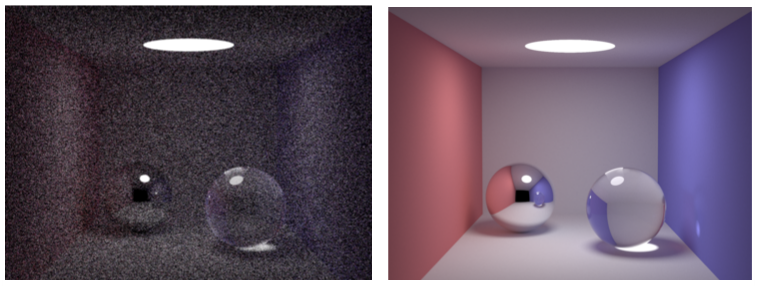
\includegraphics[width=0.8\linewidth]{images/chapter_stato_arte/stato_arte_effetto_sampling.png}\hfill
 \caption[Illuminazione al variare dei sample]{Illuminazione al variare dei sample: confronto tra render con basso valore di sample (a sinistra), e alto valore di sample (a destra).}
 \label{fig:stato_arte_effetto_sampling}
\end{figure}

È chiaro quindi quanto questo algoritmo sia computazionalmente oneroso, permettendo di ottenere risultati corretti solamente con sample alto. Maggiore è il sample, maggiore è il tempo di attesa per il completamento del rendering, migliore è il risultato dell’ illuminazione globale della scena ottenuta.
Oltre a quella appena descritta, esistono diverse implementazioni del path tracing, che permettono di ottenere alcuni vantaggi in determinate situazioni.
Un approccio prevede, quando un raggo colpisce una superficie, di lanciare un nuovo raggio sia nella direzione di rimbalzo che verso le funti di luce dirette.
\\
\begin{figure}[htb]
 \centering
 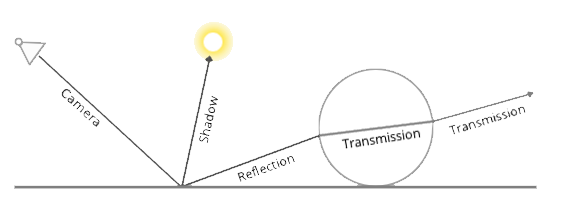
\includegraphics[width=0.8\linewidth]{images/chapter_stato_arte/stato_arte_path_alt.png}\hfill
 \caption[Path Tracing: implementazioni alternative]{Approccio utilizzato da un'implementazione alternativa dell'algoritmo di path tracing.}
 \label{fig:stato_arte_path_alt}
\end{figure}

Questa implementazione permette di ottenere in scene con poche luci indirette risultati di rendering con basso o impercettibile rumore anche con sample basso. 
Blender utilizza questo approccio con il suo Cycles Render, che verrà spiegato nei capitoli successivi.

